\documentclass[../../main.tex]{subfiles}

\begin{document}
\section{Moti su traiettoria curvilinea}
\subsection{Accelerazione tangenziale e normale}
Quando conosco la traiettoria conosco anche il versore tangente e il versore normale. Il versore tangente è diretto nella direzione della velocità e il versore normale è diretto verso la concavità della traiettoria.
\begin{figure}[h!]
    \centering
    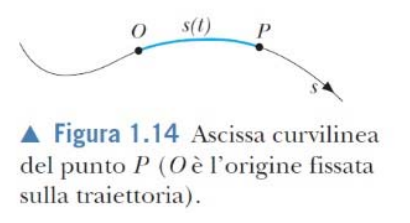
\includegraphics[width=0.5\textwidth]{curva1.png}
    \caption{$d\bar r = ds\cdot \bar u_t$}
\end{figure}
$s(t)$ è la posizione $P$, $\bar{v} = \dfrac{d\bar r}{dt} = \dfrac{ds \bar u_t}{dt} = \dfrac{ds}{dt}\bar u_t = v_s\bar u_t$ dove $v_s$ è la velocità scalare.
\begin{figure}[h!]
    \centering
    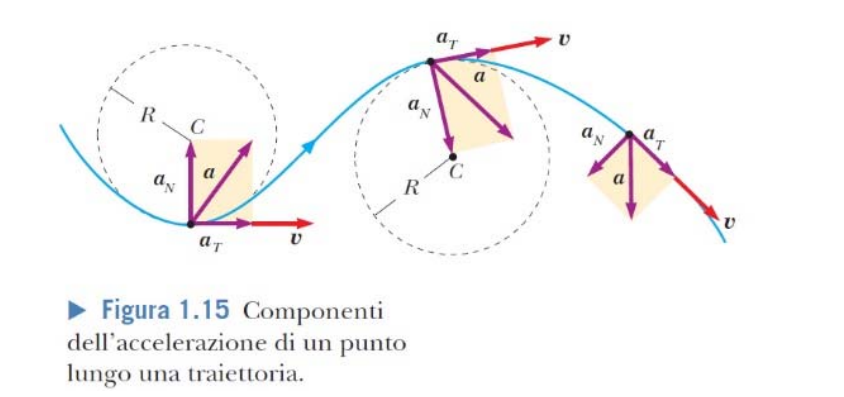
\includegraphics[width=0.5\textwidth]{curva3.png}
\end{figure}\
\[
    \bar a = \dfrac{d\bar v}{dt}
\]
\[
    \bar a_m = \dfrac{\bar v_f - \bar v_i}{\Delta t}
\]
\[
    \bar{a} = \dfrac{dv_x}{dt}\bar{u}_x + \dfrac{dv_y}{dt}\bar{u}_y + \dfrac{dv_z}{dt}\bar{u}_z = a_x\bar{u}_x + a_y\bar{u}_y + a_z\bar{u}_z
\]
\begin{minipage}{0.5\textwidth}
    \centering
    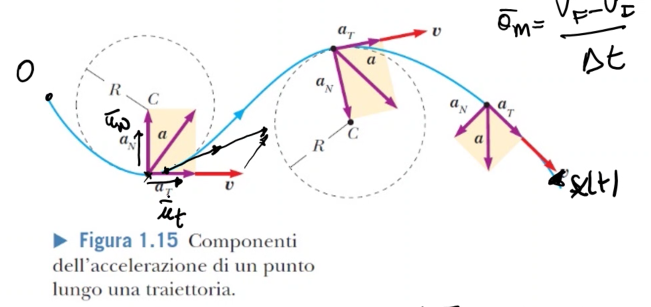
\includegraphics[width=\textwidth]{curva4.png}
    $\bar u_n$ è diretto verso la concavità
\end{minipage}
\begin{minipage}{0.5\textwidth}
    \textbf{Cerchio osculatore:} è il cerchio che meglio approssima la traiettoria in un punto. Più la curva è piana più il cerchio osculatore è grande e viceversa.
\end{minipage}
\begin{minipage}{0.5\textwidth}
    \centering
    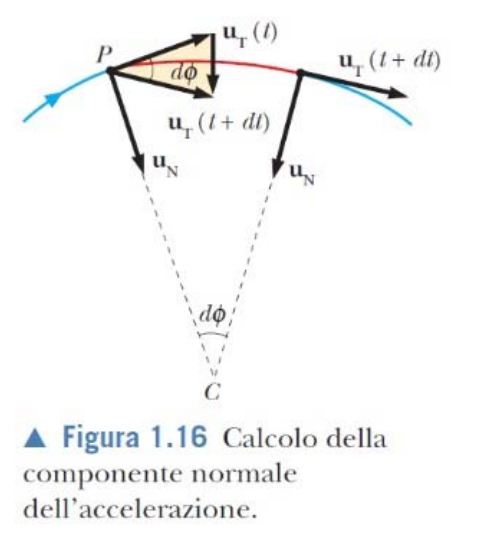
\includegraphics[width=0.5\textwidth]{curva2.png}
\end{minipage}
\begin{minipage}{0.5\textwidth}
    \centering
    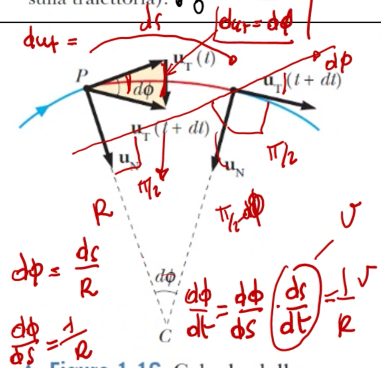
\includegraphics[width=0.5\textwidth]{curva2appunti.png}
\end{minipage}

\[
    \bar a = \dfrac{d(v \bar u_t)}{dt} = \dfrac{dv}{dt}\bar u_t + v\dfrac{d\bar u_t}{dt} = \bar a_t + v\dfrac{d_\phi \cdot \bar u_n}{dt} = \dfrac{dv}{dt}\bar{u}_t + \dfrac{v^2}{R}\bar{u}_n
\]

\subsection{Accelerazione centripeta}
vedi cosa è l'accelerazione centripeta, centra con il vettore perpendicolare al punto.
\begin{minipage}{0.5\textwidth}
    \centering
    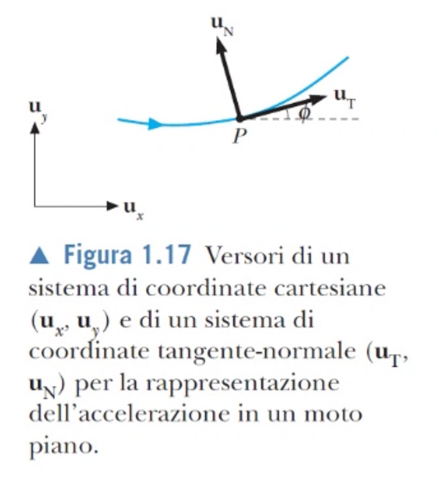
\includegraphics[width=0.5\textwidth]{centripeta.png}
\end{minipage}
\begin{minipage}{0.5\textwidth}
    $\bar v = v_s \bar u_t = \dfrac{ds}{dt}\bar u_t \\
        \bar a = \dfrac{dv_s}{dt}\bar u_t + \dfrac{v^2}{R}\bar u_n$
\end{minipage}
\vspace*{2pt}
\begin{minipage}{0.5\textwidth}
    \centering
    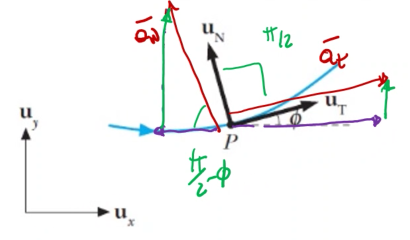
\includegraphics[width=0.5\textwidth]{centripeta2.png}
\end{minipage}
\begin{minipage}{0.5\textwidth}
    \[
        \bar r = x(t) \bar u_x + y(t) \bar u_y
    \]
    \[
        \bar v = \dfrac{d\bar x}{dt}\bar u_x + \dfrac{d\bar y}{dt}\bar u_y
    \]
    \[
        \bar a = \dfrac{d\bar v}{dt} = \dfrac{d^2\bar x}{dt^2}\bar u_x + \dfrac{d^2\bar y}{dt^2}\bar u_y + \ldots
    \]
    \[
        \bar a_x = a_x \cdot \bar{u}_x
    \]
    $\begin{cases}
            a_x = \dfrac{dv_s}{dt}\cdot \cos(\phi) - \dfrac{v^2}{R}\cdot\cos(\pi/2 - \theta) = \dfrac{dv_s}{dt} - \dfrac{v^2}{R}\cdot\sin(\phi) \\
            a_y = \dfrac{dv_s}{dt}\cdot \sin(\phi) + \dfrac{v^2}{R}\cdot\sin(\pi/2 - \theta) = \dfrac{dv_s}{dt} + \dfrac{v^2}{R}\cdot\cos(\phi)
        \end{cases}$
    $\begin{cases}
            v_x = v_s\cdot \cos(\phi) \\
            v_y = v_s\cdot \sin(\phi)
        \end{cases}$
\end{minipage}




\end{document}